\documentclass{standalone}
\usepackage{tikz}
\usetikzlibrary{patterns, positioning}


\begin{document}
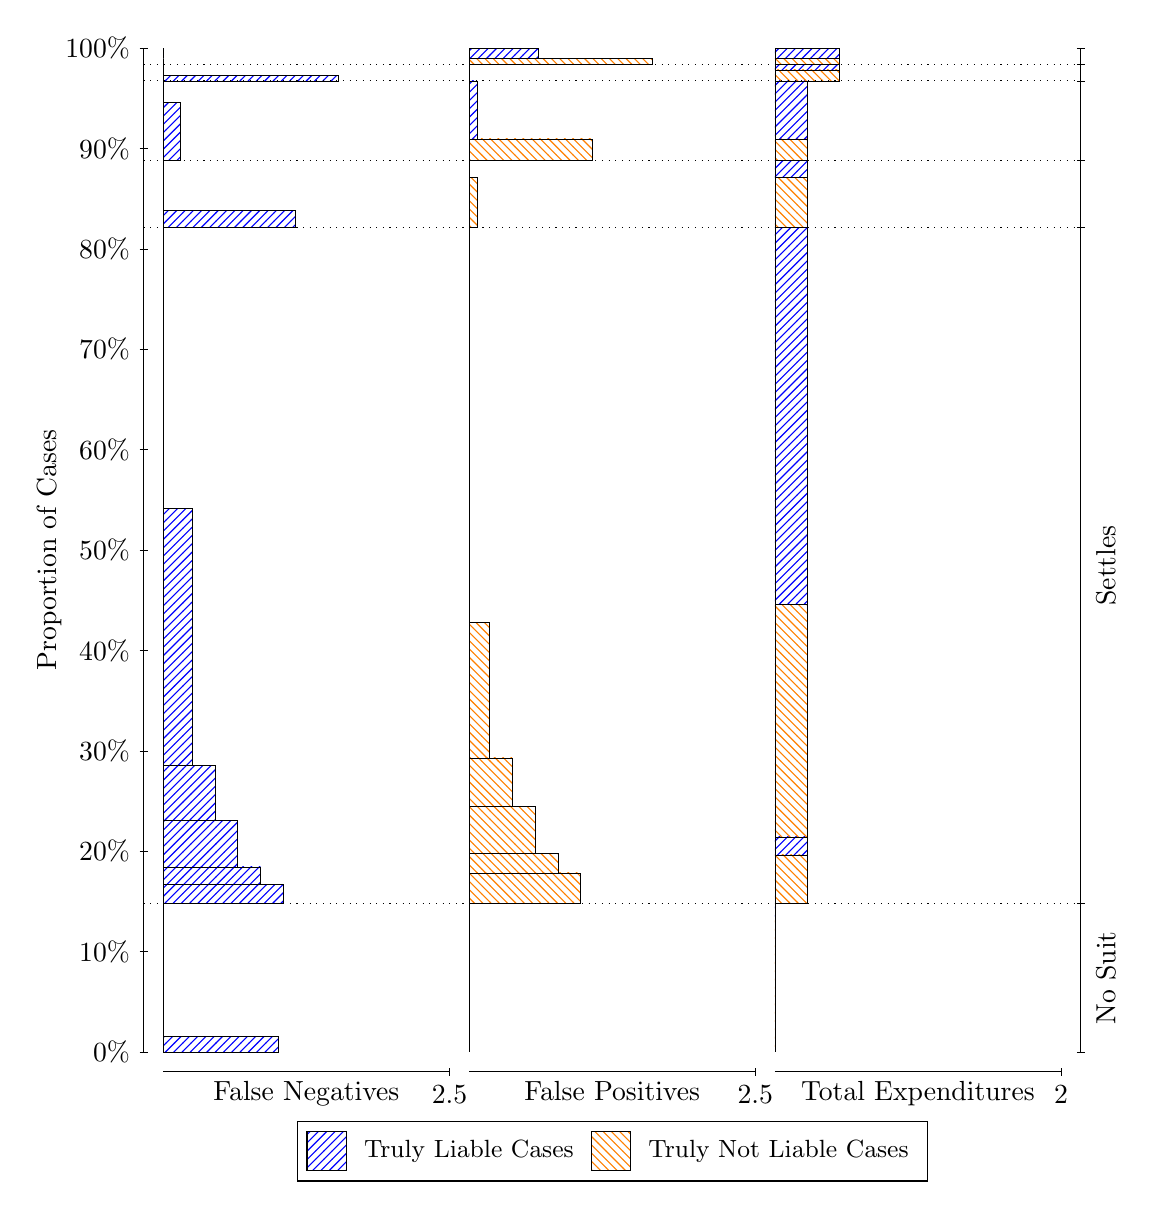
\begin{tikzpicture}
\draw[black, very thin] (1.5,1.75) -- (1.5,14.5);
\node[rotate=90, text=black, anchor=center] at (0.3, 8.125) {Proportion of Cases};
\draw[black, very thin] (1.45,1.75) -- (1.55,1.75);
\node[text=black, anchor=east] at (1.45, 1.75) {0\%};
\draw[black, very thin] (1.45,3.025) -- (1.55,3.025);
\node[text=black, anchor=east] at (1.45, 3.025) {10\%};
\draw[black, very thin] (1.45,4.3) -- (1.55,4.3);
\node[text=black, anchor=east] at (1.45, 4.3) {20\%};
\draw[black, very thin] (1.45,5.575) -- (1.55,5.575);
\node[text=black, anchor=east] at (1.45, 5.575) {30\%};
\draw[black, very thin] (1.45,6.85) -- (1.55,6.85);
\node[text=black, anchor=east] at (1.45, 6.85) {40\%};
\draw[black, very thin] (1.45,8.125) -- (1.55,8.125);
\node[text=black, anchor=east] at (1.45, 8.125) {50\%};
\draw[black, very thin] (1.45,9.4) -- (1.55,9.4);
\node[text=black, anchor=east] at (1.45, 9.4) {60\%};
\draw[black, very thin] (1.45,10.675) -- (1.55,10.675);
\node[text=black, anchor=east] at (1.45, 10.675) {70\%};
\draw[black, very thin] (1.45,11.95) -- (1.55,11.95);
\node[text=black, anchor=east] at (1.45, 11.95) {80\%};
\draw[black, very thin] (1.45,13.225) -- (1.55,13.225);
\node[text=black, anchor=east] at (1.45, 13.225) {90\%};
\draw[black, very thin] (1.45,14.5) -- (1.55,14.5);
\node[text=black, anchor=east] at (1.45, 14.5) {100\%};

\draw[black, very thin] (13.4,1.75) -- (13.4,14.5);
\draw[black, very thin] (13.35,1.75) -- (13.45,1.75);
\node[anchor=west] at (13.35, 1.75) {};
\draw[black, very thin] (13.35,3.6348) -- (13.45,3.6348);
\node[anchor=west] at (13.35, 3.6348) {};
\draw[black, very thin] (13.35,12.222) -- (13.45,12.222);
\node[anchor=west] at (13.35, 12.222) {};
\draw[black, very thin] (13.35,13.072) -- (13.45,13.072);
\node[anchor=west] at (13.35, 13.072) {};
\draw[black, very thin] (13.35,14.083) -- (13.45,14.083);
\node[anchor=west] at (13.35, 14.083) {};
\draw[black, very thin] (13.35,14.295) -- (13.45,14.295);
\node[anchor=west] at (13.35, 14.295) {};
\draw[black, very thin] (13.35,14.5) -- (13.45,14.5);
\node[anchor=west] at (13.35, 14.5) {};

\draw[black, very thin, pattern color=blue, pattern=north east lines] (1.75,1.75) rectangle (3.2033,1.9483);
\draw[black, very thin, pattern color=orange, pattern=north west lines] (1.75,1.9483) rectangle (1.75,3.6348);
\draw[black, very thin, pattern color=blue, pattern=north east lines] (1.75,3.6348) rectangle (3.276,3.8754);
\draw[black, very thin, pattern color=blue, pattern=north east lines] (1.75,3.8754) rectangle (2.9853,4.1017);
\draw[black, very thin, pattern color=blue, pattern=north east lines] (1.75,4.1017) rectangle (2.6947,4.6873);
\draw[black, very thin, pattern color=blue, pattern=north east lines] (1.75,4.6873) rectangle (2.404,5.3901);
\draw[black, very thin, pattern color=blue, pattern=north east lines] (1.75,5.3901) rectangle (2.1133,8.6538);
\draw[black, very thin, pattern color=orange, pattern=north west lines] (1.75,8.6538) rectangle (1.75,12.222);
\draw[black, very thin, pattern color=blue, pattern=north east lines] (1.75,12.222) rectangle (3.4213,12.438);
\draw[black, very thin, pattern color=orange, pattern=north west lines] (1.75,12.438) rectangle (1.75,13.072);
\draw[black, very thin, pattern color=blue, pattern=north east lines] (1.75,13.072) rectangle (1.968,13.809);
\draw[black, very thin, pattern color=orange, pattern=north west lines] (1.75,13.809) rectangle (1.75,14.083);
\draw[black, very thin, pattern color=blue, pattern=north east lines] (1.75,14.083) rectangle (3.9663,14.157);
\draw[black, very thin, pattern color=orange, pattern=north west lines] (1.75,14.157) rectangle (1.75,14.295);
\draw[black, very thin, pattern color=orange, pattern=north west lines] (1.75,14.295) rectangle (1.75,14.368);
\draw[black, very thin, pattern color=blue, pattern=north east lines] (1.75,14.368) rectangle (1.75,14.5);
\draw[black, very thin, pattern color=orange, pattern=north west lines] (5.6333,1.75) rectangle (5.6333,3.4365);
\draw[black, very thin, pattern color=blue, pattern=north east lines] (5.6333,3.4365) rectangle (5.6333,3.6348);
\draw[black, very thin, pattern color=orange, pattern=north west lines] (5.6333,3.6348) rectangle (7.0503,4.0235);
\draw[black, very thin, pattern color=orange, pattern=north west lines] (5.6333,4.0235) rectangle (6.7597,4.27);
\draw[black, very thin, pattern color=orange, pattern=north west lines] (5.6333,4.27) rectangle (6.469,4.8651);
\draw[black, very thin, pattern color=orange, pattern=north west lines] (5.6333,4.8651) rectangle (6.1783,5.4844);
\draw[black, very thin, pattern color=orange, pattern=north west lines] (5.6333,5.4844) rectangle (5.8877,7.2032);
\draw[black, very thin, pattern color=blue, pattern=north east lines] (5.6333,7.2032) rectangle (5.6333,12.222);
\draw[black, very thin, pattern color=orange, pattern=north west lines] (5.6333,12.222) rectangle (5.7423,12.857);
\draw[black, very thin, pattern color=blue, pattern=north east lines] (5.6333,12.857) rectangle (5.6333,13.072);
\draw[black, very thin, pattern color=orange, pattern=north west lines] (5.6333,13.072) rectangle (7.1957,13.347);
\draw[black, very thin, pattern color=blue, pattern=north east lines] (5.6333,13.347) rectangle (5.7423,14.083);
\draw[black, very thin, pattern color=orange, pattern=north west lines] (5.6333,14.083) rectangle (5.6333,14.221);
\draw[black, very thin, pattern color=blue, pattern=north east lines] (5.6333,14.221) rectangle (5.6333,14.295);
\draw[black, very thin, pattern color=orange, pattern=north west lines] (5.6333,14.295) rectangle (7.9587,14.368);
\draw[black, very thin, pattern color=blue, pattern=north east lines] (5.6333,14.368) rectangle (6.5053,14.5);
\draw[black, very thin, pattern color=orange, pattern=north west lines] (9.5167,1.75) rectangle (9.5167,3.4365);
\draw[black, very thin, pattern color=blue, pattern=north east lines] (9.5167,3.4365) rectangle (9.5167,3.6348);
\draw[black, very thin, pattern color=orange, pattern=north west lines] (9.5167,3.6348) rectangle (9.9254,4.2541);
\draw[black, very thin, pattern color=blue, pattern=north east lines] (9.5167,4.2541) rectangle (9.9254,4.4803);
\draw[black, very thin, pattern color=orange, pattern=north west lines] (9.5167,4.4803) rectangle (9.9254,7.4294);
\draw[black, very thin, pattern color=blue, pattern=north east lines] (9.5167,7.4294) rectangle (9.9254,12.222);
\draw[black, very thin, pattern color=orange, pattern=north west lines] (9.5167,12.222) rectangle (9.9254,12.857);
\draw[black, very thin, pattern color=blue, pattern=north east lines] (9.5167,12.857) rectangle (9.9254,13.072);
\draw[black, very thin, pattern color=orange, pattern=north west lines] (9.5167,13.072) rectangle (9.9254,13.347);
\draw[black, very thin, pattern color=blue, pattern=north east lines] (9.5167,13.347) rectangle (9.9254,14.083);
\draw[black, very thin, pattern color=orange, pattern=north west lines] (9.5167,14.083) rectangle (10.334,14.221);
\draw[black, very thin, pattern color=blue, pattern=north east lines] (9.5167,14.221) rectangle (10.334,14.295);
\draw[black, very thin, pattern color=orange, pattern=north west lines] (9.5167,14.295) rectangle (10.334,14.368);
\draw[black, very thin, pattern color=blue, pattern=north east lines] (9.5167,14.368) rectangle (10.334,14.5);
\draw[black, dotted] (1.5,3.6348) -- (13.4,3.6348);
\draw[black, dotted] (1.5,12.222) -- (13.4,12.222);
\draw[black, dotted] (1.5,13.072) -- (13.4,13.072);
\draw[black, dotted] (1.5,14.083) -- (13.4,14.083);
\draw[black, dotted] (1.5,14.295) -- (13.4,14.295);
\draw[black, very thin] (1.75,1.5) -- (5.3833,1.5);
\node[text=black, anchor=north] at (3.5667, 1.5) {False Negatives};
\draw[black, very thin] (5.3833,1.45) -- (5.3833,1.55);
\node[text=black, anchor=north] at (5.3833, 1.45) {2.5};

\draw[black, very thin] (5.6333,1.5) -- (9.2667,1.5);
\node[text=black, anchor=north] at (7.45, 1.5) {False Positives};
\draw[black, very thin] (9.2667,1.45) -- (9.2667,1.55);
\node[text=black, anchor=north] at (9.2667, 1.45) {2.5};

\draw[black, very thin] (9.5167,1.5) -- (13.15,1.5);
\node[text=black, anchor=north] at (11.333, 1.5) {Total Expenditures};
\draw[black, very thin] (13.15,1.45) -- (13.15,1.55);
\node[text=black, anchor=north] at (13.15, 1.45) {2};

\node[text=black, centered, rotate=90] at (13.72, 2.6924) {No Suit};
\node[text=black, centered, rotate=90] at (13.72, 7.9285) {Settles};





\draw (7.449999999999999,1.5) node[draw=none] (baseCoordinate) {};
\begin{scope}[align=center]
        \matrix[scale=0.5, draw=black, below=0.5cm of baseCoordinate, nodes={draw}, column sep=0.1cm]{
            \node[rectangle, draw, minimum width=0.5cm, minimum height=0.5cm, pattern color=blue, pattern=north east lines] {}; &
            \node[draw=none, font=\small, text=black] (B) {Truly Liable Cases}; &
            \node[rectangle, draw, minimum width=0.5cm, minimum height=0.5cm, pattern color=orange, pattern=north west lines] {}; &
            \node[draw=none, font=\small, text=black] (B) {Truly Not Liable Cases}; \\
            };
\end{scope}

\end{tikzpicture}
\end{document}